% Created by tikzDevice version 0.12.6 on 2024-06-11 19:56:29
% !TEX encoding = UTF-8 Unicode
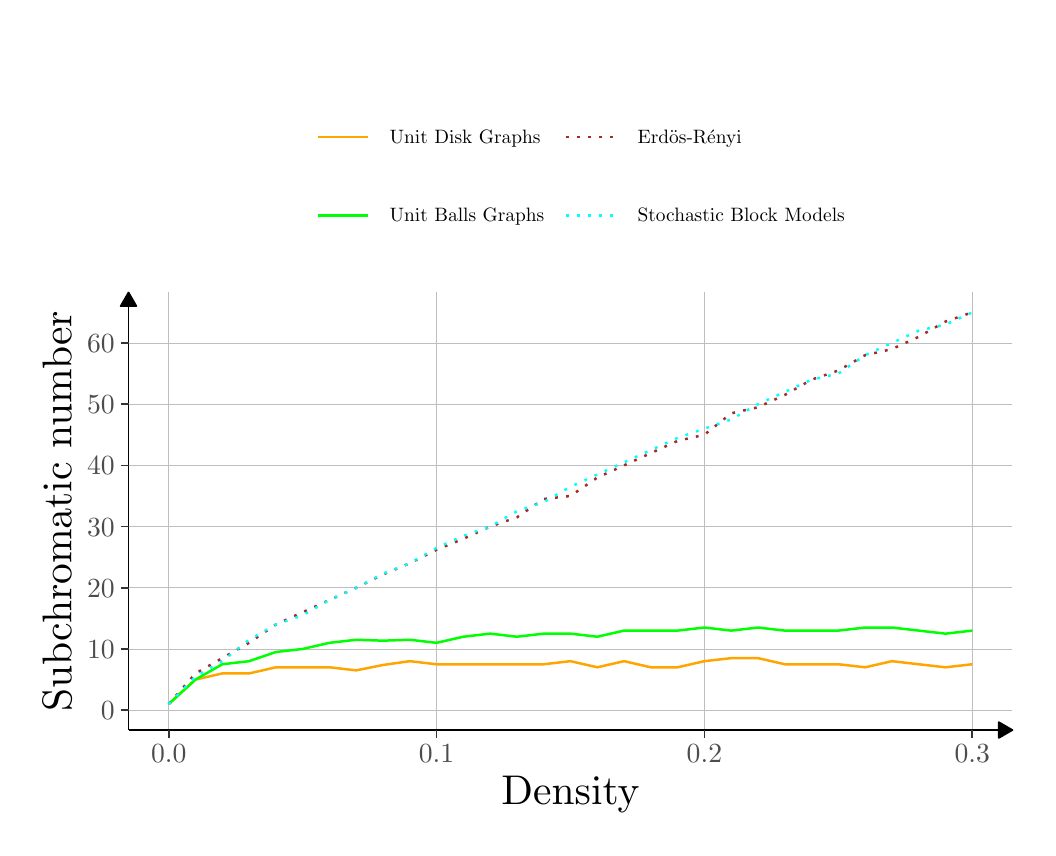
\begin{tikzpicture}[x=1pt,y=1pt]
\definecolor{fillColor}{RGB}{255,255,255}
\path[use as bounding box,fill=fillColor,fill opacity=0.00] (0,0) rectangle (361.35,289.08);
\begin{scope}
\path[clip] (  0.00,  0.00) rectangle (361.35,289.08);
\definecolor{drawColor}{RGB}{255,255,255}
\definecolor{fillColor}{RGB}{255,255,255}

\path[draw=drawColor,line width= 0.6pt,line join=round,line cap=round,fill=fillColor] (  0.00,  0.00) rectangle (361.35,289.08);
\end{scope}
\begin{scope}
\path[clip] ( 36.44, 35.28) rectangle (355.85,193.40);
\definecolor{fillColor}{RGB}{255,255,255}

\path[fill=fillColor] ( 36.44, 35.28) rectangle (355.85,193.40);
\definecolor{drawColor}{RGB}{190,190,190}

\path[draw=drawColor,line width= 0.3pt,line join=round] ( 36.44, 42.47) --
	(355.85, 42.47);

\path[draw=drawColor,line width= 0.3pt,line join=round] ( 36.44, 64.58) --
	(355.85, 64.58);

\path[draw=drawColor,line width= 0.3pt,line join=round] ( 36.44, 86.69) --
	(355.85, 86.69);

\path[draw=drawColor,line width= 0.3pt,line join=round] ( 36.44,108.81) --
	(355.85,108.81);

\path[draw=drawColor,line width= 0.3pt,line join=round] ( 36.44,130.92) --
	(355.85,130.92);

\path[draw=drawColor,line width= 0.3pt,line join=round] ( 36.44,153.04) --
	(355.85,153.04);

\path[draw=drawColor,line width= 0.3pt,line join=round] ( 36.44,175.15) --
	(355.85,175.15);

\path[draw=drawColor,line width= 0.3pt,line join=round] ( 50.96, 35.28) --
	( 50.96,193.40);

\path[draw=drawColor,line width= 0.3pt,line join=round] (147.75, 35.28) --
	(147.75,193.40);

\path[draw=drawColor,line width= 0.3pt,line join=round] (244.54, 35.28) --
	(244.54,193.40);

\path[draw=drawColor,line width= 0.3pt,line join=round] (341.33, 35.28) --
	(341.33,193.40);
\definecolor{drawColor}{RGB}{255,165,0}

\path[draw=drawColor,line width= 0.9pt,line join=round] ( 50.96, 44.68) --
	( 60.64, 53.52) --
	( 70.32, 55.73) --
	( 80.00, 55.73) --
	( 89.68, 57.95) --
	( 99.36, 57.95) --
	(109.04, 57.95) --
	(118.72, 56.84) --
	(128.39, 58.79) --
	(138.07, 60.16) --
	(147.75, 59.05) --
	(157.43, 59.05) --
	(167.11, 59.05) --
	(176.79, 59.05) --
	(186.47, 59.05) --
	(196.15, 60.16) --
	(205.83, 57.95) --
	(215.51, 60.16) --
	(225.18, 57.95) --
	(234.86, 57.95) --
	(244.54, 60.16) --
	(254.22, 61.26) --
	(263.90, 61.26) --
	(273.58, 59.05) --
	(283.26, 59.05) --
	(292.94, 59.05) --
	(302.62, 57.95) --
	(312.29, 60.16) --
	(321.97, 59.05) --
	(331.65, 57.95) --
	(341.33, 59.05);
\definecolor{drawColor}{RGB}{0,255,0}

\path[draw=drawColor,line width= 0.9pt,line join=round] ( 50.96, 44.68) --
	( 60.64, 53.52) --
	( 70.32, 59.05) --
	( 80.00, 60.16) --
	( 89.68, 63.47) --
	( 99.36, 64.58) --
	(109.04, 66.79) --
	(118.72, 67.90) --
	(128.39, 67.57) --
	(138.07, 67.90) --
	(147.75, 66.79) --
	(157.43, 69.00) --
	(167.11, 70.11) --
	(176.79, 69.00) --
	(186.47, 70.11) --
	(196.15, 70.11) --
	(205.83, 69.00) --
	(215.51, 71.21) --
	(225.18, 71.21) --
	(234.86, 71.21) --
	(244.54, 72.32) --
	(254.22, 71.21) --
	(263.90, 72.32) --
	(273.58, 71.21) --
	(283.26, 71.21) --
	(292.94, 71.21) --
	(302.62, 72.32) --
	(312.29, 72.32) --
	(321.97, 71.21) --
	(331.65, 70.11) --
	(341.33, 71.21);
\definecolor{drawColor}{RGB}{165,42,42}

\path[draw=drawColor,line width= 0.9pt,dash pattern=on 1pt off 3pt ,line join=round] ( 50.96, 44.68) --
	( 60.64, 55.73) --
	( 70.32, 61.26) --
	( 80.00, 66.79) --
	( 89.68, 73.43) --
	( 99.36, 77.85) --
	(109.04, 82.27) --
	(118.72, 86.69) --
	(128.39, 91.51) --
	(138.07, 95.54) --
	(147.75,100.42) --
	(157.43,104.39) --
	(167.11,108.81) --
	(176.79,112.13) --
	(186.47,118.76) --
	(196.15,119.87) --
	(205.83,126.50) --
	(215.51,130.92) --
	(225.18,135.35) --
	(234.86,139.77) --
	(244.54,141.98) --
	(254.22,149.72) --
	(263.90,151.93) --
	(273.58,156.36) --
	(283.26,161.88) --
	(292.94,165.20) --
	(302.62,170.73) --
	(312.29,172.94) --
	(321.97,177.37) --
	(331.65,182.89) --
	(341.33,186.21);
\definecolor{drawColor}{RGB}{0,255,255}

\path[draw=drawColor,line width= 0.9pt,dash pattern=on 1pt off 3pt ,line join=round] ( 50.96, 44.68) --
	( 60.64, 54.63) --
	( 70.32, 60.16) --
	( 80.00, 67.90) --
	( 89.68, 73.43) --
	( 99.36, 76.74) --
	(109.04, 82.27) --
	(118.72, 86.69) --
	(128.39, 91.79) --
	(138.07, 95.54) --
	(147.75,101.09) --
	(157.43,105.49) --
	(167.11,108.81) --
	(176.79,114.34) --
	(186.47,117.66) --
	(196.15,123.18) --
	(205.83,127.61) --
	(215.51,132.03) --
	(225.18,136.45) --
	(234.86,140.88) --
	(244.54,144.19) --
	(254.22,147.51) --
	(263.90,153.04) --
	(273.58,157.46) --
	(283.26,161.88) --
	(292.94,164.10) --
	(302.62,170.73) --
	(312.29,175.15) --
	(321.97,179.58) --
	(331.65,181.79) --
	(341.33,186.21);
\end{scope}
\begin{scope}
\path[clip] (  0.00,  0.00) rectangle (361.35,289.08);
\definecolor{drawColor}{RGB}{0,0,0}

\path[draw=drawColor,line width= 0.6pt,line join=round] ( 36.44, 35.28) --
	( 36.44,193.40);
\definecolor{fillColor}{RGB}{0,0,0}

\path[draw=drawColor,line width= 0.6pt,line join=round,fill=fillColor] ( 39.29,188.47) --
	( 36.44,193.40) --
	( 33.60,188.47) --
	cycle;
\end{scope}
\begin{scope}
\path[clip] (  0.00,  0.00) rectangle (361.35,289.08);
\definecolor{drawColor}{gray}{0.30}

\node[text=drawColor,anchor=base east,inner sep=0pt, outer sep=0pt, scale=  1.00] at ( 31.49, 39.02) {0};

\node[text=drawColor,anchor=base east,inner sep=0pt, outer sep=0pt, scale=  1.00] at ( 31.49, 61.14) {10};

\node[text=drawColor,anchor=base east,inner sep=0pt, outer sep=0pt, scale=  1.00] at ( 31.49, 83.25) {20};

\node[text=drawColor,anchor=base east,inner sep=0pt, outer sep=0pt, scale=  1.00] at ( 31.49,105.37) {30};

\node[text=drawColor,anchor=base east,inner sep=0pt, outer sep=0pt, scale=  1.00] at ( 31.49,127.48) {40};

\node[text=drawColor,anchor=base east,inner sep=0pt, outer sep=0pt, scale=  1.00] at ( 31.49,149.60) {50};

\node[text=drawColor,anchor=base east,inner sep=0pt, outer sep=0pt, scale=  1.00] at ( 31.49,171.71) {60};
\end{scope}
\begin{scope}
\path[clip] (  0.00,  0.00) rectangle (361.35,289.08);
\definecolor{drawColor}{gray}{0.20}

\path[draw=drawColor,line width= 0.6pt,line join=round] ( 33.69, 42.47) --
	( 36.44, 42.47);

\path[draw=drawColor,line width= 0.6pt,line join=round] ( 33.69, 64.58) --
	( 36.44, 64.58);

\path[draw=drawColor,line width= 0.6pt,line join=round] ( 33.69, 86.69) --
	( 36.44, 86.69);

\path[draw=drawColor,line width= 0.6pt,line join=round] ( 33.69,108.81) --
	( 36.44,108.81);

\path[draw=drawColor,line width= 0.6pt,line join=round] ( 33.69,130.92) --
	( 36.44,130.92);

\path[draw=drawColor,line width= 0.6pt,line join=round] ( 33.69,153.04) --
	( 36.44,153.04);

\path[draw=drawColor,line width= 0.6pt,line join=round] ( 33.69,175.15) --
	( 36.44,175.15);
\end{scope}
\begin{scope}
\path[clip] (  0.00,  0.00) rectangle (361.35,289.08);
\definecolor{drawColor}{RGB}{0,0,0}

\path[draw=drawColor,line width= 0.6pt,line join=round] ( 36.44, 35.28) --
	(355.85, 35.28);
\definecolor{fillColor}{RGB}{0,0,0}

\path[draw=drawColor,line width= 0.6pt,line join=round,fill=fillColor] (350.92, 32.43) --
	(355.85, 35.28) --
	(350.92, 38.12) --
	cycle;
\end{scope}
\begin{scope}
\path[clip] (  0.00,  0.00) rectangle (361.35,289.08);
\definecolor{drawColor}{gray}{0.20}

\path[draw=drawColor,line width= 0.6pt,line join=round] ( 50.96, 32.53) --
	( 50.96, 35.28);

\path[draw=drawColor,line width= 0.6pt,line join=round] (147.75, 32.53) --
	(147.75, 35.28);

\path[draw=drawColor,line width= 0.6pt,line join=round] (244.54, 32.53) --
	(244.54, 35.28);

\path[draw=drawColor,line width= 0.6pt,line join=round] (341.33, 32.53) --
	(341.33, 35.28);
\end{scope}
\begin{scope}
\path[clip] (  0.00,  0.00) rectangle (361.35,289.08);
\definecolor{drawColor}{gray}{0.30}

\node[text=drawColor,anchor=base,inner sep=0pt, outer sep=0pt, scale=  1.00] at ( 50.96, 23.44) {0.0};

\node[text=drawColor,anchor=base,inner sep=0pt, outer sep=0pt, scale=  1.00] at (147.75, 23.44) {0.1};

\node[text=drawColor,anchor=base,inner sep=0pt, outer sep=0pt, scale=  1.00] at (244.54, 23.44) {0.2};

\node[text=drawColor,anchor=base,inner sep=0pt, outer sep=0pt, scale=  1.00] at (341.33, 23.44) {0.3};
\end{scope}
\begin{scope}
\path[clip] (  0.00,  0.00) rectangle (361.35,289.08);
\definecolor{drawColor}{RGB}{0,0,0}

\node[text=drawColor,anchor=base,inner sep=0pt, outer sep=0pt, scale=  1.50] at (196.15,  8.42) {Density};
\end{scope}
\begin{scope}
\path[clip] (  0.00,  0.00) rectangle (361.35,289.08);
\definecolor{drawColor}{RGB}{0,0,0}

\node[text=drawColor,rotate= 90.00,anchor=base,inner sep=0pt, outer sep=0pt, scale=  1.50] at ( 15.83,114.34) {Subchromatic number};
\end{scope}
\begin{scope}
\path[clip] (  0.00,  0.00) rectangle (361.35,289.08);
\definecolor{fillColor}{RGB}{255,255,255}

\path[fill=fillColor] ( 91.55,204.40) rectangle (300.74,266.42);
\end{scope}
\begin{scope}
\path[clip] (  0.00,  0.00) rectangle (361.35,289.08);
\definecolor{fillColor}{RGB}{255,255,255}

\path[fill=fillColor] (102.55,238.16) rectangle (125.32,260.92);
\end{scope}
\begin{scope}
\path[clip] (  0.00,  0.00) rectangle (361.35,289.08);
\definecolor{drawColor}{RGB}{255,165,0}

\path[draw=drawColor,line width= 0.9pt,line join=round] (104.83,249.54) -- (123.04,249.54);
\end{scope}
\begin{scope}
\path[clip] (  0.00,  0.00) rectangle (361.35,289.08);
\definecolor{fillColor}{RGB}{255,255,255}

\path[fill=fillColor] (102.55,209.90) rectangle (125.32,232.66);
\end{scope}
\begin{scope}
\path[clip] (  0.00,  0.00) rectangle (361.35,289.08);
\definecolor{drawColor}{RGB}{0,255,0}

\path[draw=drawColor,line width= 0.9pt,line join=round] (104.83,221.28) -- (123.04,221.28);
\end{scope}
\begin{scope}
\path[clip] (  0.00,  0.00) rectangle (361.35,289.08);
\definecolor{fillColor}{RGB}{255,255,255}

\path[fill=fillColor] (192.16,238.16) rectangle (214.92,260.92);
\end{scope}
\begin{scope}
\path[clip] (  0.00,  0.00) rectangle (361.35,289.08);
\definecolor{drawColor}{RGB}{165,42,42}

\path[draw=drawColor,line width= 0.9pt,dash pattern=on 1pt off 3pt ,line join=round] (194.43,249.54) -- (212.64,249.54);
\end{scope}
\begin{scope}
\path[clip] (  0.00,  0.00) rectangle (361.35,289.08);
\definecolor{fillColor}{RGB}{255,255,255}

\path[fill=fillColor] (192.16,209.90) rectangle (214.92,232.66);
\end{scope}
\begin{scope}
\path[clip] (  0.00,  0.00) rectangle (361.35,289.08);
\definecolor{drawColor}{RGB}{0,255,255}

\path[draw=drawColor,line width= 0.9pt,dash pattern=on 1pt off 3pt ,line join=round] (194.43,221.28) -- (212.64,221.28);
\end{scope}
\begin{scope}
\path[clip] (  0.00,  0.00) rectangle (361.35,289.08);
\definecolor{drawColor}{RGB}{0,0,0}

\node[text=drawColor,anchor=base west,inner sep=0pt, outer sep=0pt, scale=  0.70] at (130.82,247.13) {Unit Disk Graphs};
\end{scope}
\begin{scope}
\path[clip] (  0.00,  0.00) rectangle (361.35,289.08);
\definecolor{drawColor}{RGB}{0,0,0}

\node[text=drawColor,anchor=base west,inner sep=0pt, outer sep=0pt, scale=  0.70] at (130.82,218.87) {Unit Balls Graphs};
\end{scope}
\begin{scope}
\path[clip] (  0.00,  0.00) rectangle (361.35,289.08);
\definecolor{drawColor}{RGB}{0,0,0}

\node[text=drawColor,anchor=base west,inner sep=0pt, outer sep=0pt, scale=  0.70] at (220.42,247.13) {Erdös-Rényi};
\end{scope}
\begin{scope}
\path[clip] (  0.00,  0.00) rectangle (361.35,289.08);
\definecolor{drawColor}{RGB}{0,0,0}

\node[text=drawColor,anchor=base west,inner sep=0pt, outer sep=0pt, scale=  0.70] at (220.42,218.87) {Stochastic Block Models};
\end{scope}
\end{tikzpicture}
